% -----------------------------------------------
% Template for ISMIR Papers
% 2016 version, based on previous ISMIR templates

% Requirements :
% * 6+1 page length maximum
% * 2MB maximum file size
% * Copyright note must appear in the bottom left corner of first page
% (see conference website for additional details)
% -----------------------------------------------

\documentclass{article}
\usepackage{ismir,amsmath,cite}
\usepackage{graphicx}
\usepackage{color}

% ------
\title{Good-sounds.org: a framework to explore goodness in instrumental sounds}

% ------------
\multauthor
{Giuseppe Bandiera$^1$ \hspace{1cm} Oriol Romani Picas$^1$ \hspace{1cm} Hiroshi Tokuda$^2$} { \bfseries{Wataru Hariya$^2$ \hspace{1cm} Koji Oishi$^2$ \hspace{1cm} Xavier Serra$^1$}\\
  $^1$ Music Technology Group, Universitat Pompeu Fabra, Barcelona, Spain\\
$^2$ Technology Development Dept., KORG Inc., Tokyo, Japan\\
{\tt\small giuseppe.bandiera@upf.edu, oriol.romani@upf.edu}
}
\def\authorname{Giuseppe Bandiera, Oriol Romani Picas, Hiroshi Tokuda, Wataru Hariya, Koji Oishi, Xavier Serra}

%\threeauthors
%  {First Author} {Affiliation1 \\ {\tt author1@ismir.edu}}
%  {Second Author} {\bf Retain these fake authors in\\\bf submission to preserve the formatting}
%  {Third Author} {Affiliation3 \\ {\tt author3@ismir.edu}}


\sloppy % please retain sloppy command for improved formatting

\begin{document}

%
\maketitle
%
\begin{abstract}
We introduce good-sounds.org, a community driven framework to explore the concept of goodness in instrumental sounds. Goodness is considered here as the common agreed basic sound quality of an instrument without taking into consideration musical expressiveness. Musicians upload their sounds and vote on existing sounds, and from the collected data the system is able to develop sound goodness measures of relevance for music education applications. The core of the system is a database of sounds, together with audio features extracted from them and user annotations related to the goodness of the sounds. The web front-end provides useful data visualizations of the sound attributes and tools to facilitate user interaction. To evaluate the framework, we carried out an experiment to rate sound goodness of single notes of nine orchestral instruments. In it, users rated the sounds using an AB vote over a set of sound attributes defined to be of relevance in the characterization of single notes of instrumental sounds. With the obtained votes we built a ranking of the sounds for each attribute and developed a model that rates the goodness for each of the selected sound attributes. Using this approach, we have succeeded in obtaining results comparable to a model that was built from expert generated evaluations.
\end{abstract}
%
\section{Introduction}\label{sec:introduction}

Measuring sound goodness, or quality, in instrumental sounds is difficult due to its intrinsic subjectivity. Ne\-ver\-theless, it has been shown that there is some consistency among people while discriminating good or bad music performances \cite{1}. Furthermore, recent studies have demonstrated a correlation between the perceived music quality and the musical performance technique \cite{2}. Bearing this in mind, in a previous work \cite{01} we proposed a method to automatically rate goodness by defining a set of sound attributes and by using a set of good/bad labels given by expert musicians. The definition of goodness was treated as a classification problem and an outcome of that work was a mobile application (Cortosia) that gives goodness scores in real-time for single notes on a scale from 0 to 100. This score was computed considering the distribution of the features values in the classification step. While developing that system we realized that we could improve the scores, specially their correlation with the perceptual sound goodness, if we could use more training data and include a range of goodness levels given by users rather than the binary good/bad labels that we used. However, the task of labeling sounds this way would have been very time consuming and we would  also need more sounds, covering the whole range of sound goodness. To address these issues we are now crowdsourcing the problem. We have developed a website, good-sounds.org, on which users can upload sound content and can tag and rate sounds in various ways.      
%
\section{good-sounds.org}\label{sec:goodsounds}
Good-sounds.org\footnote{\textit{https://good-sounds.org}} is an online platform to explore the concept of goodness in instrumental sounds with the help of a community of users. It provides social community features in the web front-end and a framework for sound analysis and modeling in the background. It also includes an API to access the collected data.

\begin{figure}[ht]
 \centerline{\framebox{
 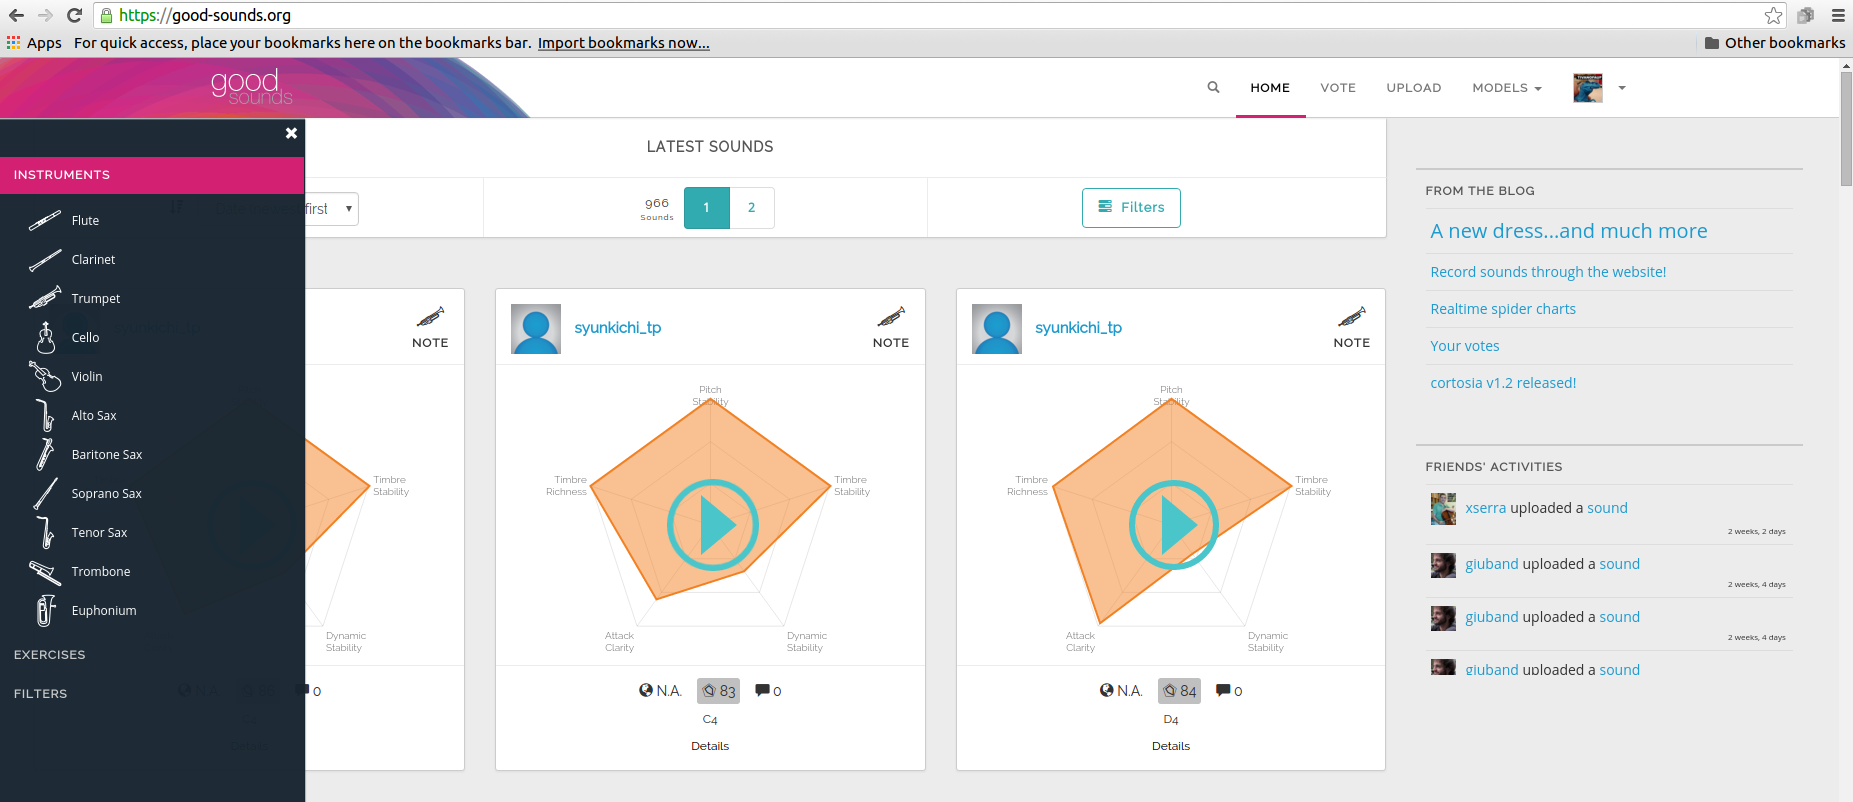
\includegraphics[width=\columnwidth]{figs/sound_list.png}}}
 \caption{Good-sound.org sound list page.}
 \label{fig:sound_list}
\end{figure}

\subsection{Description} 
The website has been designed from a user perspective, meant to be modern and to provide a seamless experience. It makes use of state of the art design concepts and community oriented web technologies. The web front-end includes three main sections: (1) a page to list and visua\-lize the uploaded sounds as shown in Figure~\ref{fig:sound_list}, (2) a page to upload and describe sounds as shown in Figure~\ref{fig:upload} and (3) a section to gather user ratings and annotations. The visualization page shows a list of all the sounds and it includes filter options to narrow down the results, being able to show things like specific instruments or sounds uploaded a certain date. The upload page allows users to add sounds into the site and also provides a recording tool built using Web Audio API\footnote{\textit{http://www.w3.org/TR/webaudio/}}. The annotation section has been designed for the specific experiment explained in Section~\ref{experiment}. 
The website backend is written in Python using the Django web application framework. The metadata is stored in a PostgreSQL database while the sound files plus other analysis files are stored locally in the server. An API accepts requests from authorized clients to upload sounds (currently through the mobile app Cortosia) and retrieve statistics from the user’s community. At this time, the website supports 11 instruments, it includes 8470 unique sounds and there are 363 active users. 

\begin{figure}
 \centerline{\framebox{
 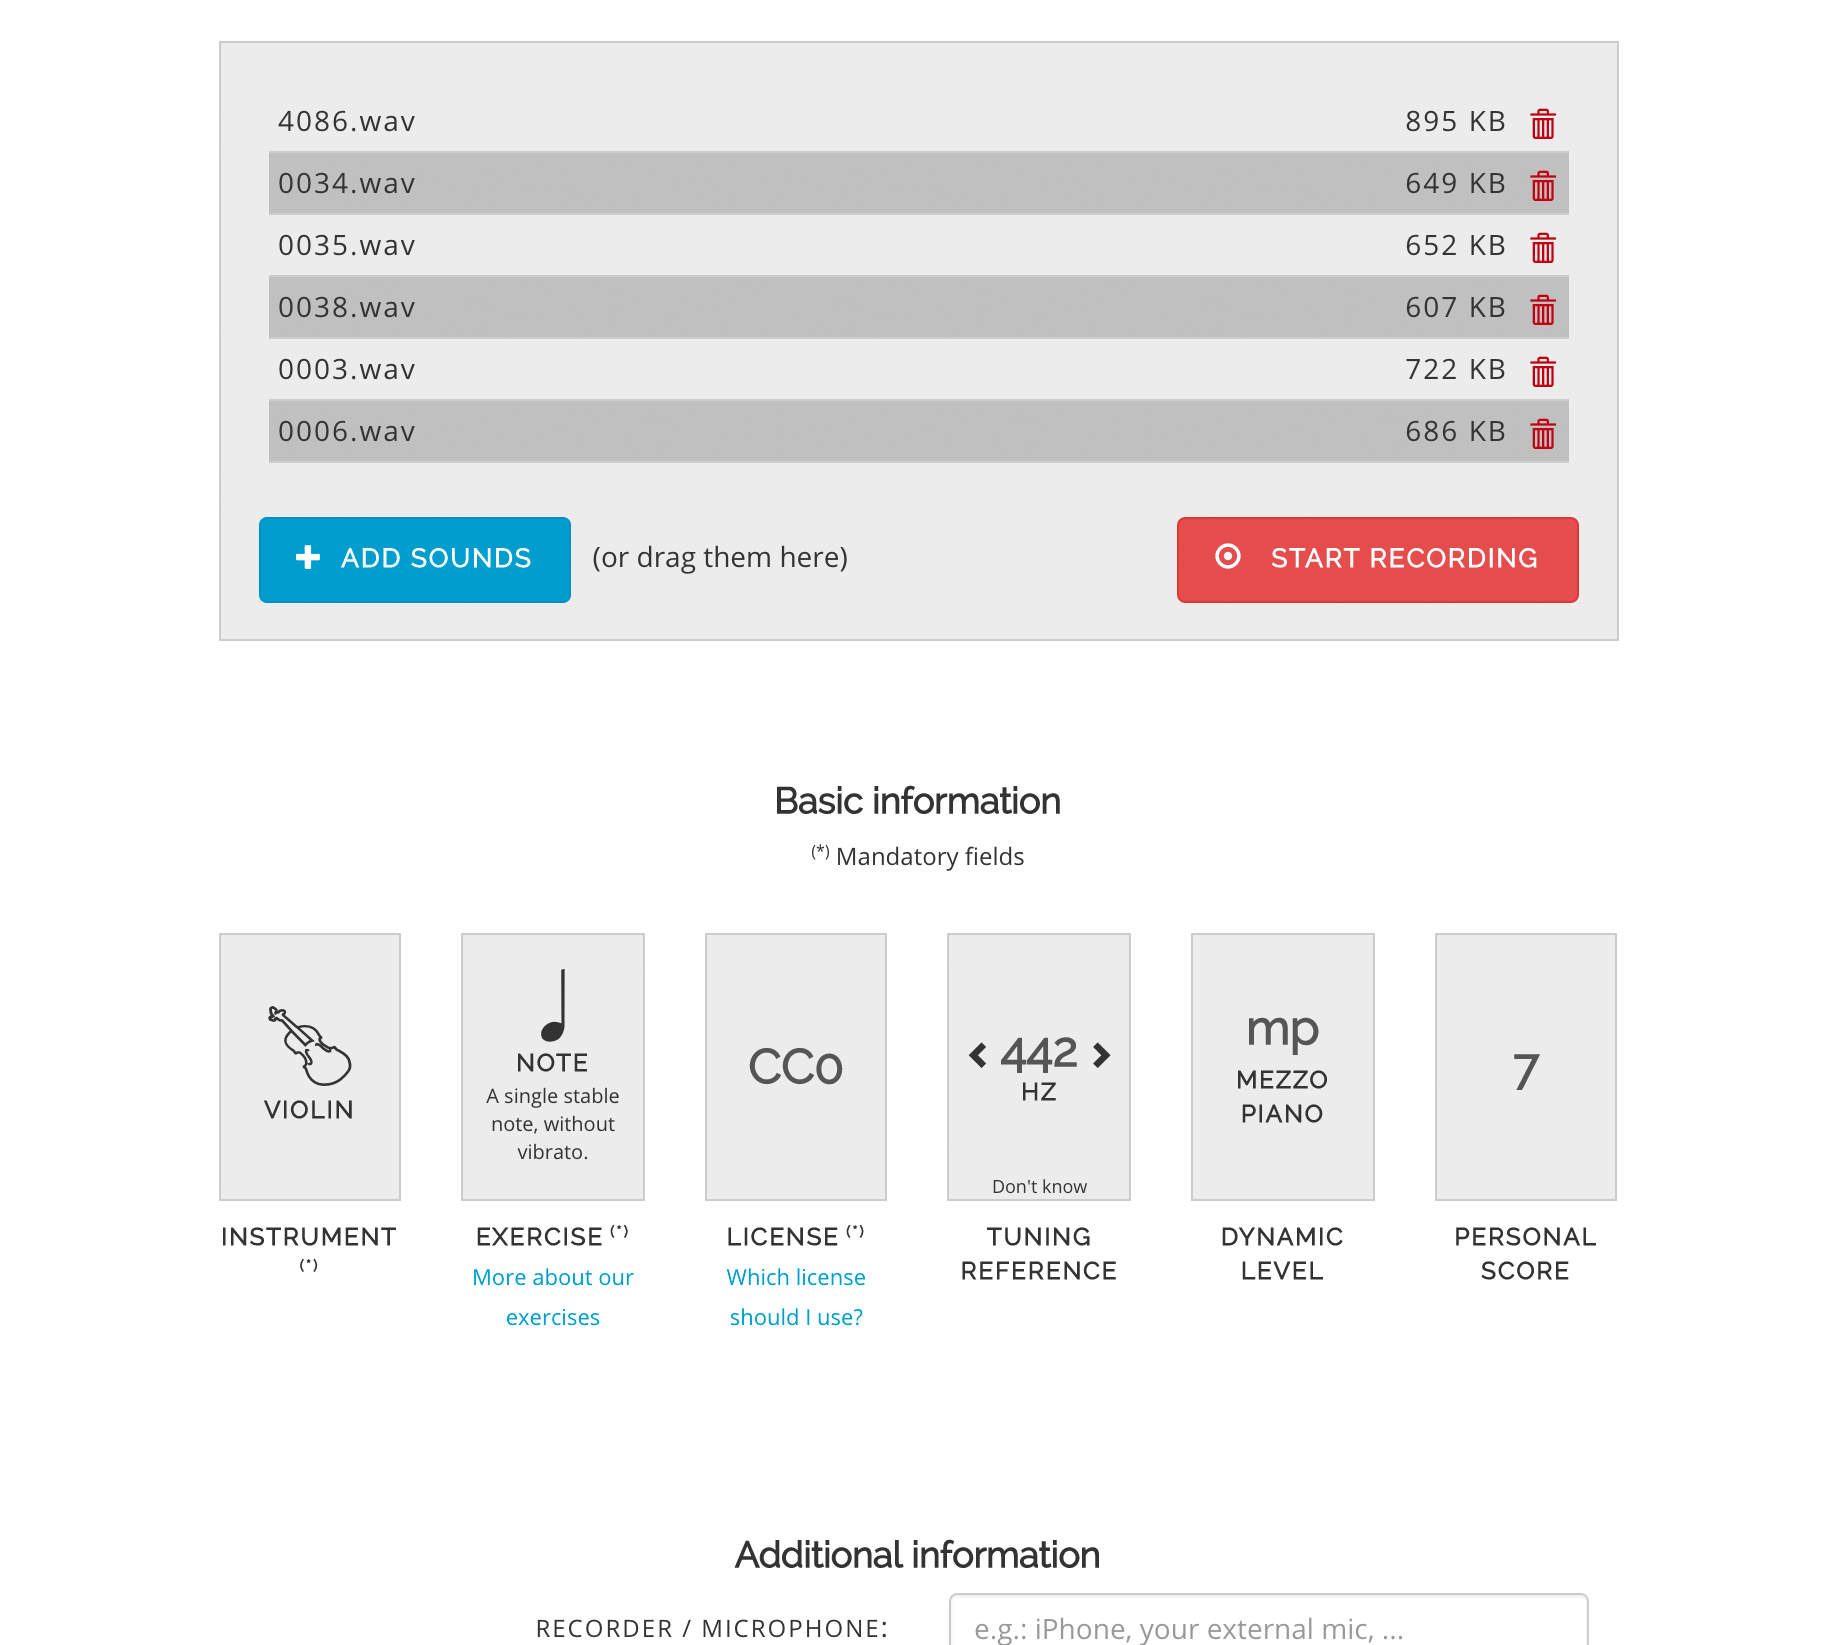
\includegraphics[width=\columnwidth]{figs/upload.png}}}
 \caption{Good-sound.org sound upload page.}
 \label{fig:upload}
\end{figure}

\subsection{Content}
The main data stored in good-sounds.org consists of sounds and the metadata accompanying them. When uploading sounds, the users can choose between three different types of Creative Commons licenses for their content: Universal, Attribution or Attribution Non-Commercial. As soon as a sound is uploaded, it is analyzed using the freesound extractor \cite{02}, thus obtaining a number of low-level audio features, and the system generates an mp3 version of the file together with images of the waveform and spectrogram. The audio, image and audio feature files are stored in the good-sounds server and the metadata is stored in the PostgreSQL database. 

\subsubsection{Segmentation}
One of the critical audio processing steps performed in good-sounds.org is the segmentation of the uploaded sound files to find appropriate note boundaries. Given that the audios come from different and not well controlled sources, they might include all kinds of issues (ex. silence at beginning and end or background noise) that can difficult the subsequent feature extraction steps. Considering that the sounds we are working with are all monophonic pitched instrument sounds, we can base the segmentation mainly on pitch. Our approach extracts pitch using Essentia’s \cite{03} implementations of the YinFFT algorithm \cite{07} and the Yin time based algorithm \cite{05}. Then the sound is segmented into notes using pitch contours \cite{06} and signal RMS with Essentia’s PitchContourSegmentation algorithm.  
The segmentation data is also stored in the database. This allows us to build client-side data visualizations that effectively reflect the quality of the segmentation algorithm and the user can modify the parameters for this algorithm and re-run it on the fly from the website. The results of this ite\-ration is immediately shown on the same page, for an easy comparison of the results, as it is shown in Figure~\ref{fig:segmentation}.

\begin{figure}[ht]
 \centerline{\framebox{
 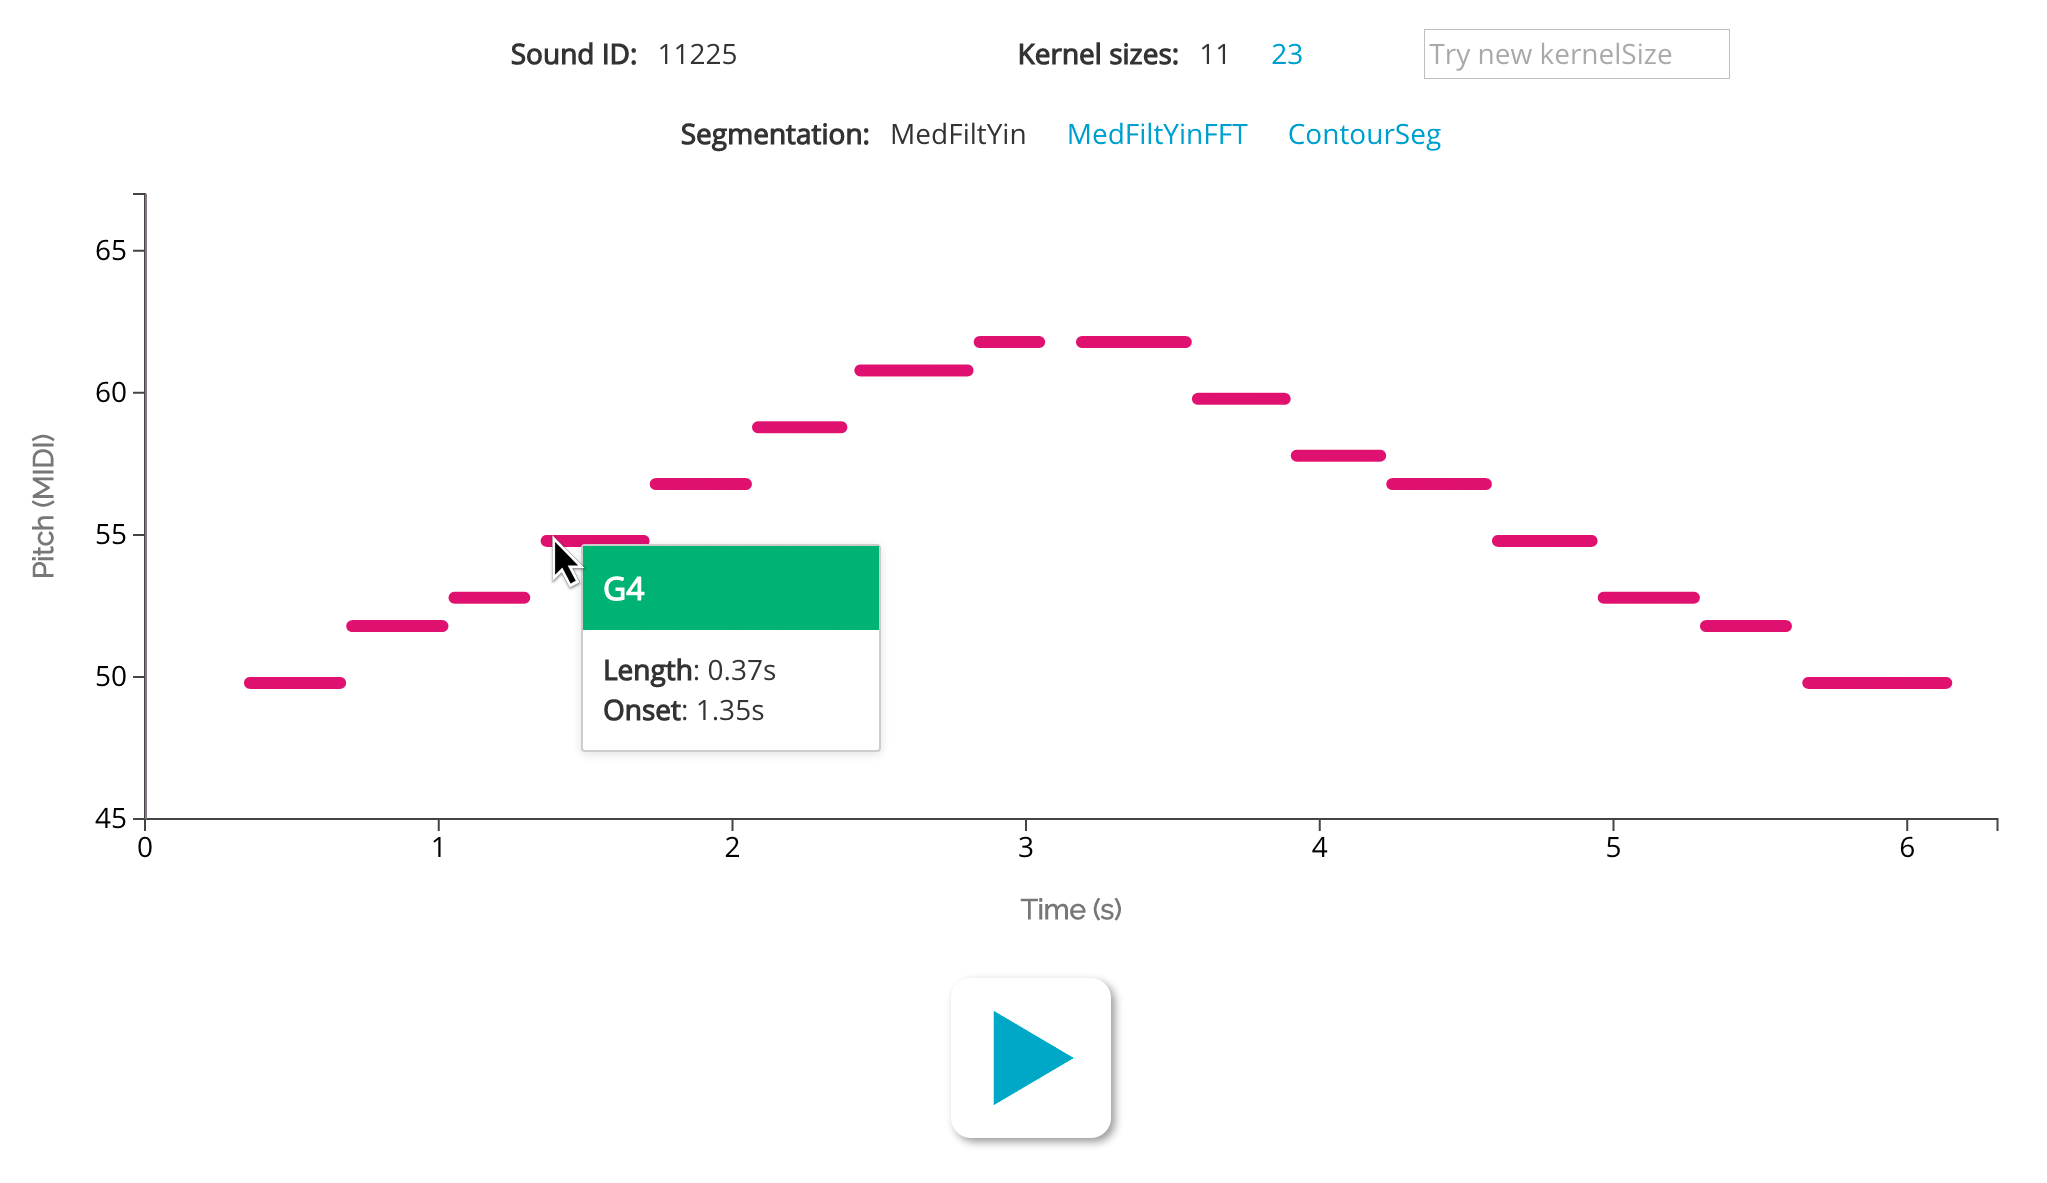
\includegraphics[width=\columnwidth]{figs/segmentation.png}}}
 \caption{Good-sound.org segmentation visualisation page.}
 \label{fig:segmentation}
\end{figure}

\subsubsection{Descriptors}
The feature extraction module (using the freesound extractor of Essentia) computes spectral, tonal and temporal descriptors. With it, the audios are first resampled to 44.1kHz sampling rate and normalised using ReplayGain\footnote{\textit{http://wiki.hydrogenaud.io/index.php?title=ReplayGain}}. The descriptors are then extracted across all the frames using a 2048 window size and 512 hop window size. We then compute statistical measures (mean, median and standard deviation) of the descriptors which are the values stored as JSON files in the server. The list of the descriptors extracted is shown in Table~\ref{table:descriptors}. 

\begin{table*}[ht]
\centering
\begin{tabular}{lll}
\hline
spectral                                                                                                                                                                                 & tonal                                      & temporal                                            \\ \hline
\begin{tabular}[c]{@{}l@{}}spectrum, barkbands, \\ melbands, flatness, crest, rolloff, \\ decrease, hfc, pitch salience, flatness db, \\skewness, kurtosis, spectral complexity,\end{tabular} & pitch yinfft, pitch yin, pitch confidence, & zerocrossingrate, loudness, centroid, \\flatness sfx, \\
\hline
\end{tabular}
\caption{Descriptors extracted by Essentia library present in good-sounds.org.}
\label{table:descriptors}
\end{table*}


\section{Experiment} \label{experiment}
As a test case to evaluate the usefulness of the good-sounds.org framework we setup an experiment to rate the goodness of single notes. The goal of the experiment was to build models from both the uploaded sounds and the community annotations, with which we can then automatically rate the sound goodness. We compared the results of the obtained models with the ones we got in our previous work using expert annotations.  

\subsection{Dataset}
The data used in this experiment comes from several sources. First, we uploaded all the sounds from our previous work to the website, together with the expert annotations. Since the website has been public for a few months, we also had  sounds uploaded by users, both directly and through the mobile app (using the API). Then, user annotations on the sounds according to a goodness scale where collected using a voting task. These annotations use a set of sound attributes that affect sound goodness. These attributes were defined in our previous article \cite{01} by consulting with a group of music experts:   
\begin{itemize}
	\item{\textit{dynamic stability}: the stability of the loudness.}
	\item{\textit{pitch stability}: the stability of the pitch.}
	\item{\textit{timbre stability}: the stability of the timbre.}
	\item{\textit{timbre richness}: the quality of the timbre.}
	\item{\textit{attack clarity}: the quality of the attack.}
\end{itemize}

\subsubsection{Sounds}
For this experiment we only used single note sounds. At the time of the experiment there were sounds for 5467 single notes of 9 instruments. We show the list of sounds per instrument in Table~\ref{sounds}. The sounds we recorded ourselves from the recording sessions are uncompressed wave files, while the ones uploaded by users to the website are in different audio formats.  

\begin{table}[ht]
\centering
\begin{tabular}{cc}
\hline
instrument   & number of sounds \\ \hline
cello        & 935              \\
violin       & 802              \\
clarinet     & 1360             \\
flute        & 1434             \\
alto sax     & 352              \\
baritone sax & 292              \\
tenor sax    & 292              \\
soprano sax  & 343              \\
trumpet      & 738              \\ \hline
\end{tabular}
\caption{Number of sounds in the experiment's dataset.}
\label{sounds}
\end{table}

\subsubsection{Annotations}
We distinguish two kinds of annotations: (1) recording annotations and (2) community annotations. The recor\-ding annotations are the ones coming from the recording sessions that we did and consists of one tag per sound. This tag says if the sound is a good or a bad example of each sound attribute (e.g. bad-timbre-stability, good-attack-clarity…). Those are the annotations used later on for a first evaluation of the models and are only available for the sounds we recorded ourselves.
The community annotations are the ones generated from the user votes and used in this work to explore goodness. In order to be able to rate a sound in a goodness scale we need annotations on a wide range of different goodness levels. We originally thought of asking the community to rate sounds in a scale of goodness but we discarded this option because of the following:

\begin{itemize}
	\item{the task can be excessively demanding.}
	\item{without a reference sound the criteria of different users can differ extremely.}
	\item{with a reference sound we influence the user’s criteria, thus annotations can be less 	generalisable.}
\end{itemize}

Instead, we designed a user task that gave as outcome a ranked list of the sounds based on the goodness for each sound attribute. An A/B multi vote task was used for this purpose. Two sounds are presented and the user is asked to decide which sound is better according to one or more of the sound attributes. One vote is stored for each selected attribute. A list of the votes per instruments (considering all sound attributes) is shown in Table~\ref{votes}.
In order to prevent random votes in the task we run checks periodically. This checks consists of two sounds; one being a bad example of a sound attribute regarding the expert annotations and the other being a good example. The task is presented to the users the first time they vote and also randomly after some votes. If the user does not vote for the expected sound in the reference task, his next votes are not used. The votes of this user are again taken into account if he succeeds to pass the reference task. 


\begin{table}[ht]
\centering
\begin{tabular}{cc}
\hline
instrument   & number of votes \\ \hline
cello        & 140             \\
violin       & 90              \\
clarinet     & 293             \\
flute        & 305             \\
alto sax     & 78              \\
baritone sax & 59              \\
tenor sax    & 14              \\
soprano sax  & 21              \\
trumpet      & 230             \\ \hline
\end{tabular}
\caption{Number of votes in good-sounds for the dataset's experiment.}
\label{votes}
\end{table}

\subsubsection{Rankings}
In order to have learning data in a wide range of goodness we built rankings with the community votes for each sound attribute. The position of a sound in the ranking represents its goodness level. To build them we count the number of wins and the number of votes of each sound in the database. Then the sounds are sorted according to two parameters: 

\begin{itemize}
	\item{total number of votes: number of participations in the voting task.}
	\item{ratio between wins and votes: the ratio between the number of wins and the total number of participations in the voting task.}
\end{itemize}
  
Using these parameters for building the rankings we assure that the sounds in the top are the ones voted more times, as being better than others, and not sounds with few votes but high percentage of wins.

\subsection{Learning}
The goal of our learning process is to build a model for each instrument that is able to rate each sound attribute in a 0 to 100 score. To do so we want to find a set of features that highly correlate with the rankings extracted in the previous step.  
Our approach uses a regression model to predict the score. These predictions are then used as samples of the final score function. The final score is then computed as an interpolation of the samples.

\subsubsection{Models}
We want to find the combination of regression model and set of features that better describes the rankings. For such a purpose we tried different regression algorithms available in scikit-learn \cite{08}.  As one of the outputs of the project is a system that rates the goodness of sounds in real-time we want to restrict the number of features in order to maintain a low computational cost. For each one of the algorithms we build a model for each ranking using one, two or three features and we compute the average prediction score of the model across all the options. The prediction score $R^2$  or Coefficient of Determination is defined as follows:

\begin{equation}
 R^2 = (1 - u/v) 
\end{equation}
where
\begin{equation}
	u = \sum\nolimits((y_{true} - y_{pred})^2)
\end{equation}
and
\begin{equation}
	v = \sum\nolimits((y_{true} - \prod\limits_{i=1}^n y_{true})^2)
\end{equation}

Where $y_{true}$ is the set of ground truth annotations and $y_{pred}$ the set of predictions, having both the same length. The best possible score $R^2$ is 1.0 and it can be negative.
The variance of the prediction score across all the rankings and set of features is also computed. 
The number of features that give the best score for each ranking is taken into account to compute an average number of features for each regression model. A comparison of the performance of the different models is shown in Table~\ref{models}.

\begin{table*}[ht]
\centering
\label{my-label}
\begin{tabular}{cccc}
\hline
Regression model  & Avg. score & Score variance & Average of features \\ \hline
SVR               & -1.208     & 5.4436         & 1.843               \\
Ridge             & -2.644     & 31.005         & 2.166               \\
KRR               & -1.79      & 10.798         & 1.906               \\
Linear regression & -3.503     & 30.03          & 1.718               \\
RANSAC            & -3.202     & 17.532         & 1.478               \\
Theilsen          & -4.14      & 37.135         & 1.781               \\ \hline
\end{tabular}
\caption{Performance of the different regression models.}
\label{models}
\end{table*}

As we can see in the table, the SVR (Epsilon-Support Vector Regression) model has the best average score across all the rankings and using all possible combination of feature sets (up to 3 features). It also has the lowest score variance so we can expect the model to be robust across the different instruments and sound attributes. However the average number of features is almost two and the computation of two features at each frame of all the sounds in the database can be computationally expensive. For this reason we tested how good the model can be if we force it to use less than three features. We show the results of such a comparison in Table~\ref{svr}.

\begin{table}[]
\centering
\label{my-label}
\begin{tabular}{lll}
\hline
Regression model & Avg. score & Score variance \\ \hline
SVR 3 features   & -1.208     & 5.4436         \\
SVR 2 features   & -1.2411    & 5.3895         \\
SVR 1 feature    & -1.4254    & 5.6554         \\ \hline
\end{tabular}
\caption{Performance of SVR model with different number of features.}
\label{svr}
\end{table}

The results show that the differences between using one or three features are not too big so we decided to use SVR with a single feature  in order to maintain a low computational cost for future applications of the system. We then tried all possible combinations of parameters (kernel, degree of polynomially, cost parameter..) to find the best model for each instrument and sound attribute.

\subsubsection{Scores}
From the model we predict the ranking position of a sound and we map this position into a 0 to 100 score of the sound attribute. The final goodness score is computed as the average score across the five attributes. We compute the sound attribute scores of all the sounds in the database to test the distribution of the scores according to the feature value. For example, a distribution of the score for the timbre stability of flute is shown in Figure~\ref{fig:scores}.

\begin{figure}[ht]
 \centerline{\framebox{
 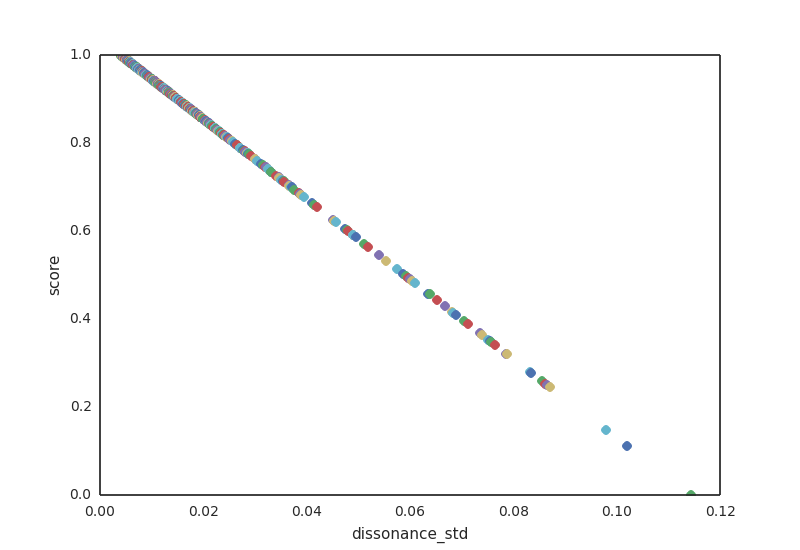
\includegraphics[width=\columnwidth]{figs/distribution_1.png}}}
 \caption{Distribution of scores of flute timbre stability.}
 \label{fig:scores}
\end{figure}

The resulting distributions are not balanced. For this reason we push the scores of each sound attribute to fit a Gaussian distribution. This gives us balanced distributions and it also allows us to refine the scores by tweaking the parameters of the gaussian function. A result of this process is shown in Figure~\ref{fig:scores_2}. The final score is computed interpolating the feature according to these tuned distributions. 

\begin{figure}[ht]
 \centerline{\framebox{
 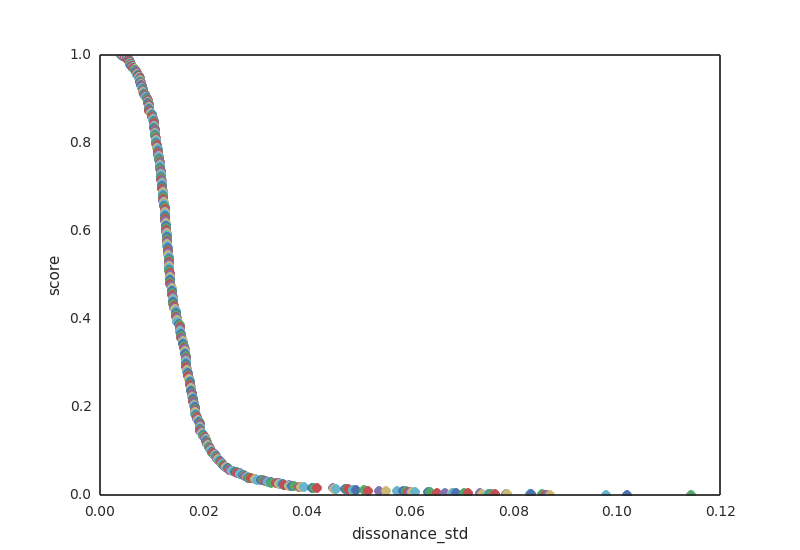
\includegraphics[width=\columnwidth]{figs/distribution_2.png}}}
 \caption{Distribution of scores of flute timbre stability after normalisation.}
 \label{fig:scores_2}
\end{figure}

\subsubsection{Models evaluation}
In order to evaluate the models we want to check the correlation between the scores and the rankings as we expect the sounds ranked in the first positions to have the highest scores. We evaluate this correlation using Kendall Rank Correlation Coefficient \cite{09}, commonly referred as Kendall’s tau coefficient. 
We use the implementation available in the scipy library, that is based on the tau-b version. Its computation, given two rankings $x$ and $y$ of the same size  is defined by the following equation:
\begin{equation}
\tau = \frac{(P - Q)} {\sqrt((P + Q + T)*(P + Q + U))}
\end{equation}
where $P$ is the number of concordant pairs, $Q$ the number of discordant pairs, $T$ the number of ties only in $x$, and $U$ the number of ties only in $y$. If a tie occurs for the same pair in both $x$ and $y$, it is not added to either $T$ or $U$.
The values range from -1 to 1, where 1 indicates strong agreement and -1 strong disagreement. 
We compute $\tau$ between the score and the ranking position for all the sounds that are contained in the rankings. 
The results for each sound attribute and instrument are shown in Table 6.


\begin{table*}[ht]
\centering
\begin{tabular}{lcccccccccc}
\hline
\textbf{Sound attribute} & \multicolumn{1}{l}{Flute} & \multicolumn{1}{l}{Violin} & \multicolumn{1}{l}{Clarinet} & \multicolumn{1}{l}{Trumpet} & \multicolumn{1}{l}{Cello} & \multicolumn{1}{l}{Violin} & \multicolumn{1}{l}{Alto sax} & \multicolumn{1}{l}{Baritone sax} & \multicolumn{1}{l}{Soprano} & \multicolumn{1}{l}{\textbf{Average}} \\ \hline
timbre stability         & 0.37                      & 0.65                       & 0.46                         & 0.38                        & 0.28                      & 0.65                       & 0.33                         & 0.73                             & 0.73                        & \textbf{0.51}                        \\
dynamic stability        & 0.41                      & 0.33                       & 0.24                         & 0.44                        & 0.64                      & 0.33                       & 0.33                         & 0.31                             & 0.31                        & \textbf{0.37}                        \\
pitch stability          & 0.42                      & 0.46                       & 0.22                         & 0.38                        & 0.58                      & 0.46                       & 1                            & 1                                & 0.81                        & \textbf{0.59}                        \\
timbre richness          & 0.04                      & 0.35                       & 0.32                         & 0.11                        & 0.21                      & 0.35                       & 1                            & 0.56                             & 1                           & \textbf{0.43}                        \\
attack clarity           & 0.33                      & 0.59                       & 0.38                         & 0.3                         & 0.18                      & 0.59                       & 0                            & 0.34                             & 0.35                        & \textbf{0.34}                        \\ \hline
\end{tabular}
\label{tau}
\caption{Kendall tau coefficient between the scores and the rankings of each sound attribute.}
\end{table*}

\section{Conclusions}
In this article we presented a web based framework for exploring sound goodness in instrumental sounds using a community of users. The framework provides an easy way to collect sounds and annotations as well as tools to extract and store music descriptors. This allows us to explore the concept of sound goodness in a controlled and flexible environment. Furthermore, the website is useful to the community as a place in which to discuss the issues affecting sound goodness as well as a learning tool to improve their playing techniques. 
As a way to evaluate the framework we extended our previous work by using annotations from the community collected through a voting task. The models built using this approach provide an automatic rating of goodness for each attribute that tends to match the expert annotations collected in our previous work. The results should improve with more annotations from the community.
As future work we want to design new tasks to collect user annotations and build new models according to them. 

\section{Acknowledgements}
This research has been partially funded by KORG Inc. The authors would like to thank the entire good-sounds.org community who contributed to the website with sounds and annotations.

% For bibtex users:
%\bibliography{ISMIRtemplate}

% For non bibtex users:
\begin{thebibliography}{citations}

\bibitem {1}
J. Geringer and C. Madsen.
``Musicians ratings of good versus bad vocal and string performances,''
{\it Journal of Research in Music Education}, vol. 46, pages 522-534, 1998.

\bibitem {2}
Brian E. Russell.
``An empirical study of a solo performance assessment model,''
{\it  International Journal of Music Education}, vol. 33, pages 359-371, 2015.

\bibitem {01}
O. Romaní Picas, H. Parra Rodriguez, D. Dabiri, H. Tokuda, W. Hariya, K. Oishi, and X. Serra.
``A real-time system for measuring sound goodness in instrumental sounds,''
{\it Audio Engineering Society Convention 138.} Audio Engineering Society 2015.

\bibitem {02}
 F. Font, G. Roma, and X. Serra.
``Freesound technical demo,''
{\it Proceedings of the 21st ACM international conference on Multimedia}, 2013.

\bibitem {03}
 D. Bogdanov, N. Wach, E. G\'omez, S. Gulati, P. Herrera, O. Mayor, G. Roma, J. Salamon, J. R. Zapata, and X. Serra.
``Essentia: An audio analysis library for music information retrieval,''
{\it  Proceedings of the International Society for Music Information Retrieval Conference,} pages 493-498, 2013.

\bibitem {05}
 A. de Cheveigné and H. Kawahara.
``YIN, a fundamental frequency estimator for speech and music,''
{\it The Journal of the Acoustical Society of America,} pages 111-1917, 2002.

\bibitem {06}
 R. J. McNab, Ll. A. Smith, and I. H. Witten.
``Signal processing for melody transcription,''
{\it Australasian Computer Science Communications 18}, pages 301-307, 1996.

\bibitem {07}
P. M. Brossier.
``Automatic Annotation of Musical Audio for Interactive Applications,''
{\it Ph.D. Thesis, Queen Mary University of London, UK}, 2007.

\bibitem {08}
F. Pedregosa, G. Varoquaux, A. Gramfort, V. Michel, B. Thirion, O. Grisel, M. Blondel, P. Prettenhofer, R. Weiss, V. Dubourg, and J. Vanderplas.
``Scikit-learn: Machine Learning in Python,''
{\it Journal of Machine Learning Research 12}, pages 2825-2830, 2011.

\bibitem {09}
Stepanov, Alexei. ``On the Kendall Correlation Coefficient," arXiv preprint arXiv:1507.01427, 2015.



\end{thebibliography}

\end{document}
